    Se desarrolló el análisis estático de la cámara MARK III para fuerzas de gravedad cuando la misma se encuentra montada en diferentes orientaciones, sea de lado o de cabeza. 
    En primer lugar, para desarrollar el análisis estático fue necesario simplificar el modelo del mecanismo de las secciones que no son relevantes para el análisis, como los dientes de los engranes por ejemplo como se aprecia en la Figura \ref{fig:configuracionSimplificada}.
    
    \begin{figure}[H]
    \centering
    \begin{adjustbox}{width=\linewidth/2} 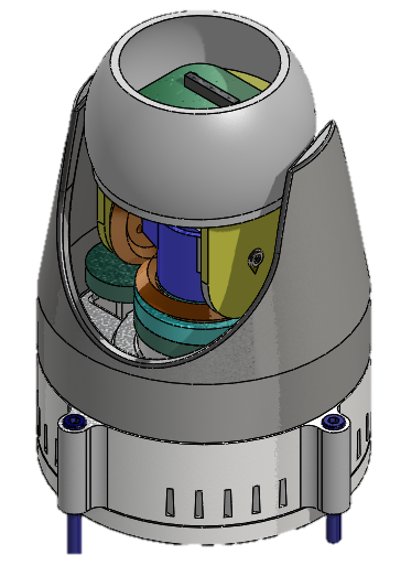
\includegraphics{media/analisisEstatico/configuracionSimplificdaSimulacion.png}
    \end{adjustbox}
    \caption{\label{fig:configuracionSimplificada}Configuración simplificada del modelo optimizada para simulación.}
    \end{figure} 
    
    Se tomó en cuenta que las cargas mas importantes del sistema son los motores, con 9.5 gramos cada uno, la placa de la cámara de 10 gramos y el conjunto de potencia con un promedio de 250 gramos y se representó estas cargas mediante fuerzas para simplificar el análisis. En la Figura \ref{fig:deformaciones_unitarias} se pueden observar tres simulaciones, una para cada orientación para las que la cámara esta diseñada a montarse. Se puede notar en la Figura que las deformaciones se encuentran dentro del limite elástico del plástico seleccionado, en este caso ABS. 
    
    \begin{figure}[H]
    \centering
    \begin{adjustbox}{width=\linewidth} 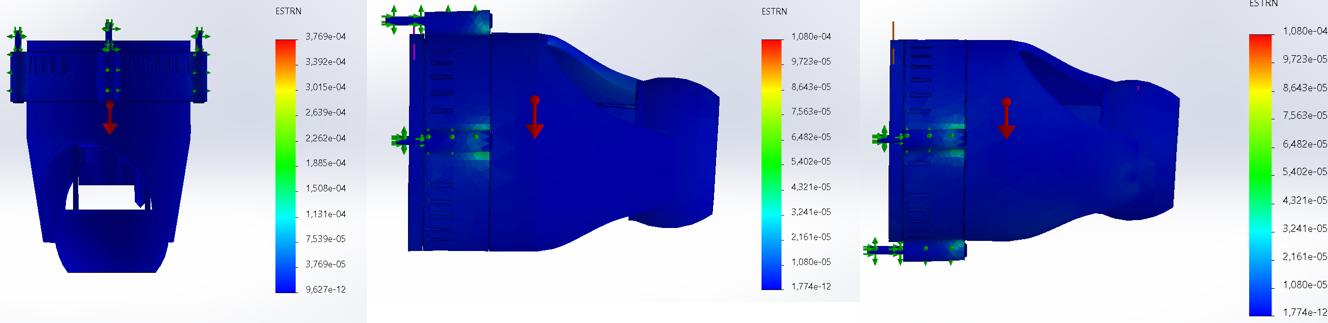
\includegraphics{media/analisisEstatico/deformacionesUnitarias123.png}
    \end{adjustbox}
    \caption{\label{fig:deformaciones_unitarias}Estudio de Deformaciones Unitarias del MARK III ante carga de la gravedad en diferentes orientaciones.}
    \end{figure} 

    Por otro lado, la Figura~\ref{fig:deformaciones_unitarias} muestra los desplazamientos, lo mas notable es que el mecanismo de la cámara tiende a desplazarse un promedio de 0.007 mm hacia la dirección de la gravedad cuando la cámara se coloca de lado.

    \begin{figure}[H]
    \centering
    \begin{adjustbox}{width=\linewidth} 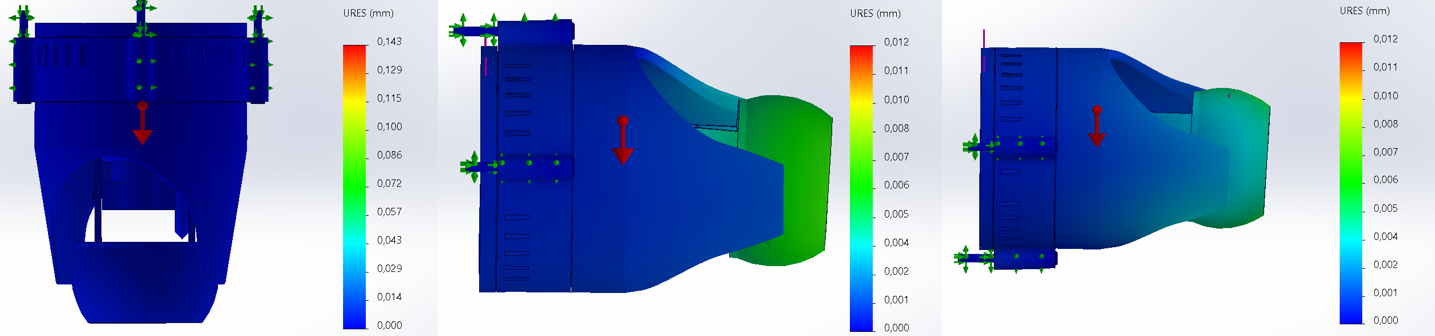
\includegraphics{media/analisisEstatico/desplazamientos123.png}
    \end{adjustbox}
    \caption{\label{fig:analisisDesplazamientos}Estudio de Desplazamientos del MARK III ante carga de la gravedad en diferentes orientaciones.}
    \end{figure} 

    La Figura~\ref{fig:analisisTensiones} permite apreciar el análisis de tensiones. Nada que destacar del análisis de tensiones.

    \begin{figure}[H]
    \centering
    \begin{adjustbox}{width=\linewidth} 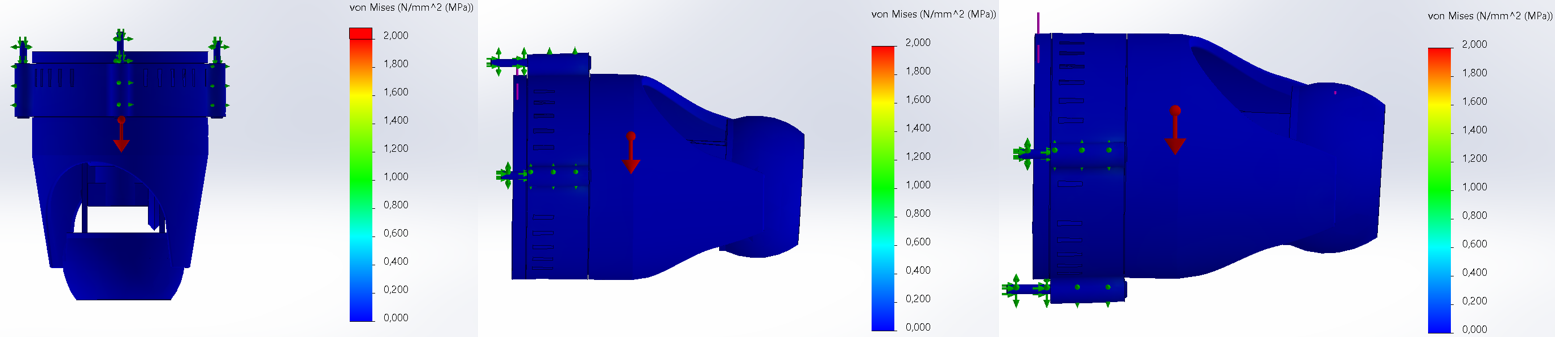
\includegraphics{media/analisisEstatico/tensiones123.png}
    \end{adjustbox}
    \caption{\label{fig:analisisTensiones}Estudio de Tensiones del MARK III ante carga de la gravedad en diferentes orientaciones.}
    \end{figure} 

    \begin{figure}[H]
    \centering
    \begin{adjustbox}{width=\linewidth} 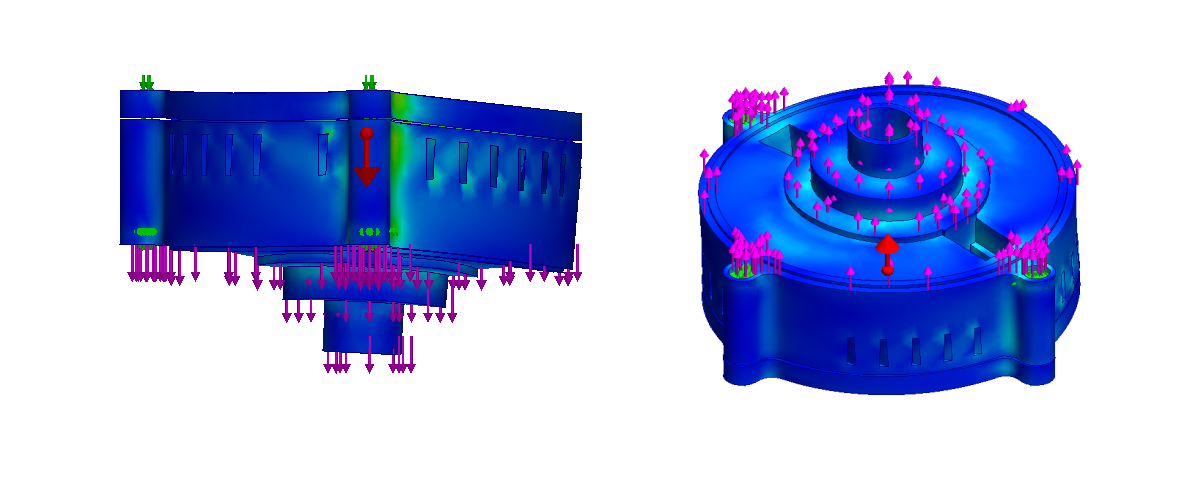
\includegraphics{media/analisisEstatico/simulacion_base.png}
    \end{adjustbox}
    \caption{\label{fig:simBase} Análisis Estático de la Base de la Cámara.}
    \end{figure} 
    
    Finalmente en la Figura~\ref{fig:simBase} se simuló la carga de la carcasa, componentes y conjunto electrónico en la carcasa, puesto que es la base de donde se sostiene la misma. Se colocó la carga distribuida en los soportes y superficies superiores de la base mientras se fijaba los soportes para pernos.